\chapter{Seleção de Correias Sincronizadoras}

Para a escolha das polias sincronizadoras são necessários os parâmetros fundamentais para correias trapezoidais citados na seção 2.

\section{Passo 01 - Definição da potência do projeto}

Com base na Figura~\ref{k0_tabela} para se obter o fator de serviço, na Eq.\eqref{9.24} se consegue calcular a potência de projeto.


\section{Passo 02 - Definição da especificação da correia}

A partir da potência e da rotação do eixo motor, é possível determinar a especificação da correia utilizando a Figura~\ref{abaco_sinc}

\begin{figure}[h]
	\centering
	\caption{Ábaco seleção de correias sincronizadoras}
    \label{abaco_sinc}
	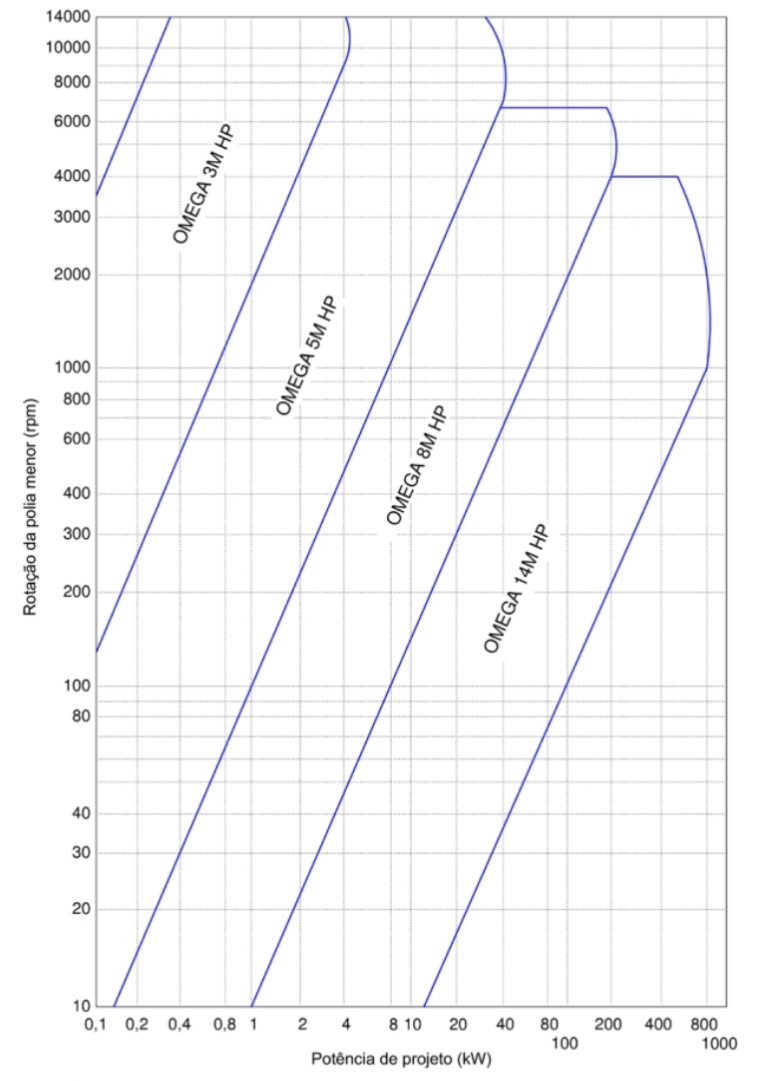
\includegraphics[scale=0.5]{Imagens/abaco_sinc.png}
	\fonte{\cite{EMA_Barbieri}}
\end{figure}

\section{Passo 03 - Definição dos números de dentes e diâmetros das polias}

Em função da potência de projeto e da rotação do eixo mais rápido, é possível definir o número de dentes mais recomendado para a polia motora, com base nas tabelas 9.10 a 9.13 de \cite{EMA_Barbieri}. Deve-se manter em mente o número mínimo de dentes recomendado para cada situação.

As tabelas de \cite{EMA_Barbieri} 9.20 a 9.23 fornecem o diâmetro das polias em função do número de dentes.

\section{Passo 04 - Definição da velocidade tangencial da correia}

Usa-se a Eq.~\eqref{v_correia} para determinar a velocidade tangencial da correia


\section{Passo 05 - Definição da distância entre eixos}

Para uma estimativa prévia da distância entre os eixos, pode-se usar as seguintes relações:

\begin{equation}
    a > 0,5(d_{p2} + d_{p1}) +15\text{mm} \qquad \text{e} \qquad a<2,0(d_{p2} + d_{p1})
\end{equation}

\section{Passo 06 - Cálculo do comprimento da correia}

Utiliza-se a Eq. \eqref{comprimento_correia} para o cálculo do comprimento da correia

\section{Passo 07 - Escolha do comprimento e correção da distância entre centros}

Efetiva-se os ajustes de comprimento com base nas Tabelas 9.14 a 9.17 de \cite{EMA_Barbieri}. O ajuste final é realizado usando a Eq. \eqref{deixo}.

\section{Passo 08 - Determinação de dentes em contato com a polia pequena}

É possível determinar a quantidade de dentes em contato com a polia pequena durante o funcionamento do sistema utilizando:

\begin{equation}
    z_e=\frac{z_1}{6} \left(3-\frac{d_{p2}-d_{p1}}{a_{corr}} \right)
\end{equation}



\section{Passo 09 - Determinação dos fatores de correção}

Como nas correias trapezoidais, fatores de correção precisam ser aplicados, são obtidos a partir das Figuras~\ref{correcao_dentes} e \ref{correcao_comp2}, com base no número de dentes em contato e o comprimento.

\begin{figure}[h]
	\centering
	\caption{Fator de correção com número de dentes}
    \label{correcao_dentes}
	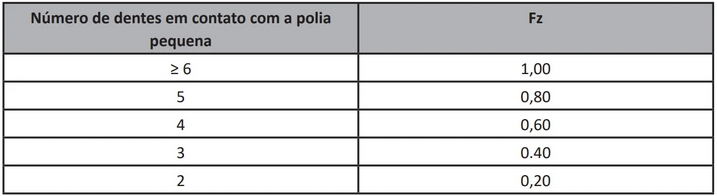
\includegraphics[scale=0.7]{Imagens/correcao_dentes.png}
	\fonte{\cite{EMA_Barbieri}}
\end{figure}

\begin{figure}[h]
	\centering
	\caption{Fator de correção com comprimento}
    \label{correcao_comp2}
	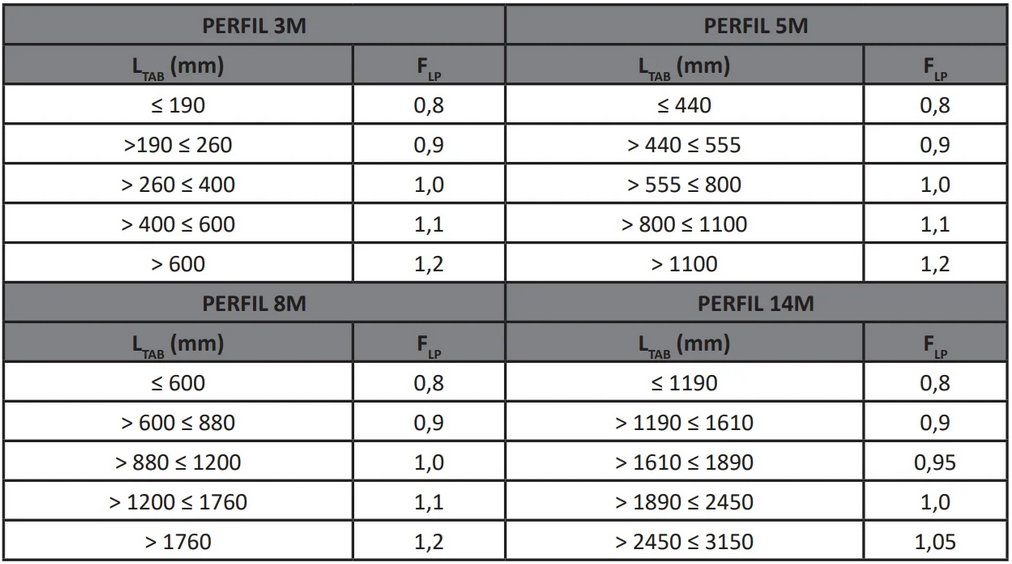
\includegraphics[scale=0.5]{Imagens/correcao_comp2.png}
	\fonte{\cite{EMA_Barbieri}}
\end{figure}

\pagebreak

\section{Passo 10 - Verificação da potência nominal da correia}

Os limites de potência nominal que as correias são capazes de transmitir estão presentes nas Tabelas 9.10 a 9.13 de \cite{EMA_Barbieri}, se encontram em função do número de dentes e da rotação. Deve-se verificar se a correia selecionada atende os requisitos do projeto, caso seja necessário deve-se selecionar uma largura de correia superior, a seguinte equação exibe essa relação.

\begin{equation}
    P_N F_{LP} F_Z \geq P_P
\end{equation}